\chapter{Methodology}
\label{chap:methodology}

This chapter presents the methodological framework used to develop \ac{RL}-based control policies for reducing \ac{NOx} emissions in the considered hybrid electric vehicle. The goal is to track a target speed trajectory closely while minimising \ac{NOx} emissions and maintaining the battery's \ac{SOC}.

The chapter first introduces the closed-loop interaction between the agent and the \ac{LSTM}-based surrogate environment, then formulates the control task as an approximate \ac{MDP} and motivates the selected observation, action, and reward design at a conceptual level. It subsequently describes the curriculum-inspired two-phase training procedure, in which speed-tracking feasibility is established before emission- and \ac{SOC}-related objectives are introduced. Finally, it defines the evaluation logic used to compare agents and to establish the baselines that later optimisation stages must improve upon.

This chapter is closely linked to the implementation details described in \autoref{chap:experimental_setup}. It explains the methodological \textit{what} and \textit{why}, allowing the overall approach to be followed and reproduced at a conceptual level. The following chapter, by contrast, addresses \textit{how exactly} the methodology was implemented and therefore supports reproducibility at an engineering level.

% ---------------------------------------------------------------------
\section{Overview — The Control Loop}
\label{sec:method_overview}
% [NEW] High-level closed loop: RL agent <-> LSTM-surrogate environment.
%  - One figure resembling the PA4 ppt flow: agent emits actions; the LSTM
%    stack returns speed / SOC / NOx / temperatures; the reward is computed
%    and fed back. Keep it concept-level (no tensor shapes / no code).
%  - [SHIFT] Bridge from Related Work: the prior project used a RECURRENT
%    TD3 + Ray, framed as a POMDP, and could not stabilise the speed; this
%    thesis steps back to NON-recurrent SB3 agents on an MDP approximation,
%    and from a single fixed target speed to tracking a full speed TRAJECTORY.
%  - State the chapter roadmap: frame the problem -> two-phase procedure ->
%    evaluation methodology.

\begin{figure}[htbp]
  \centering
  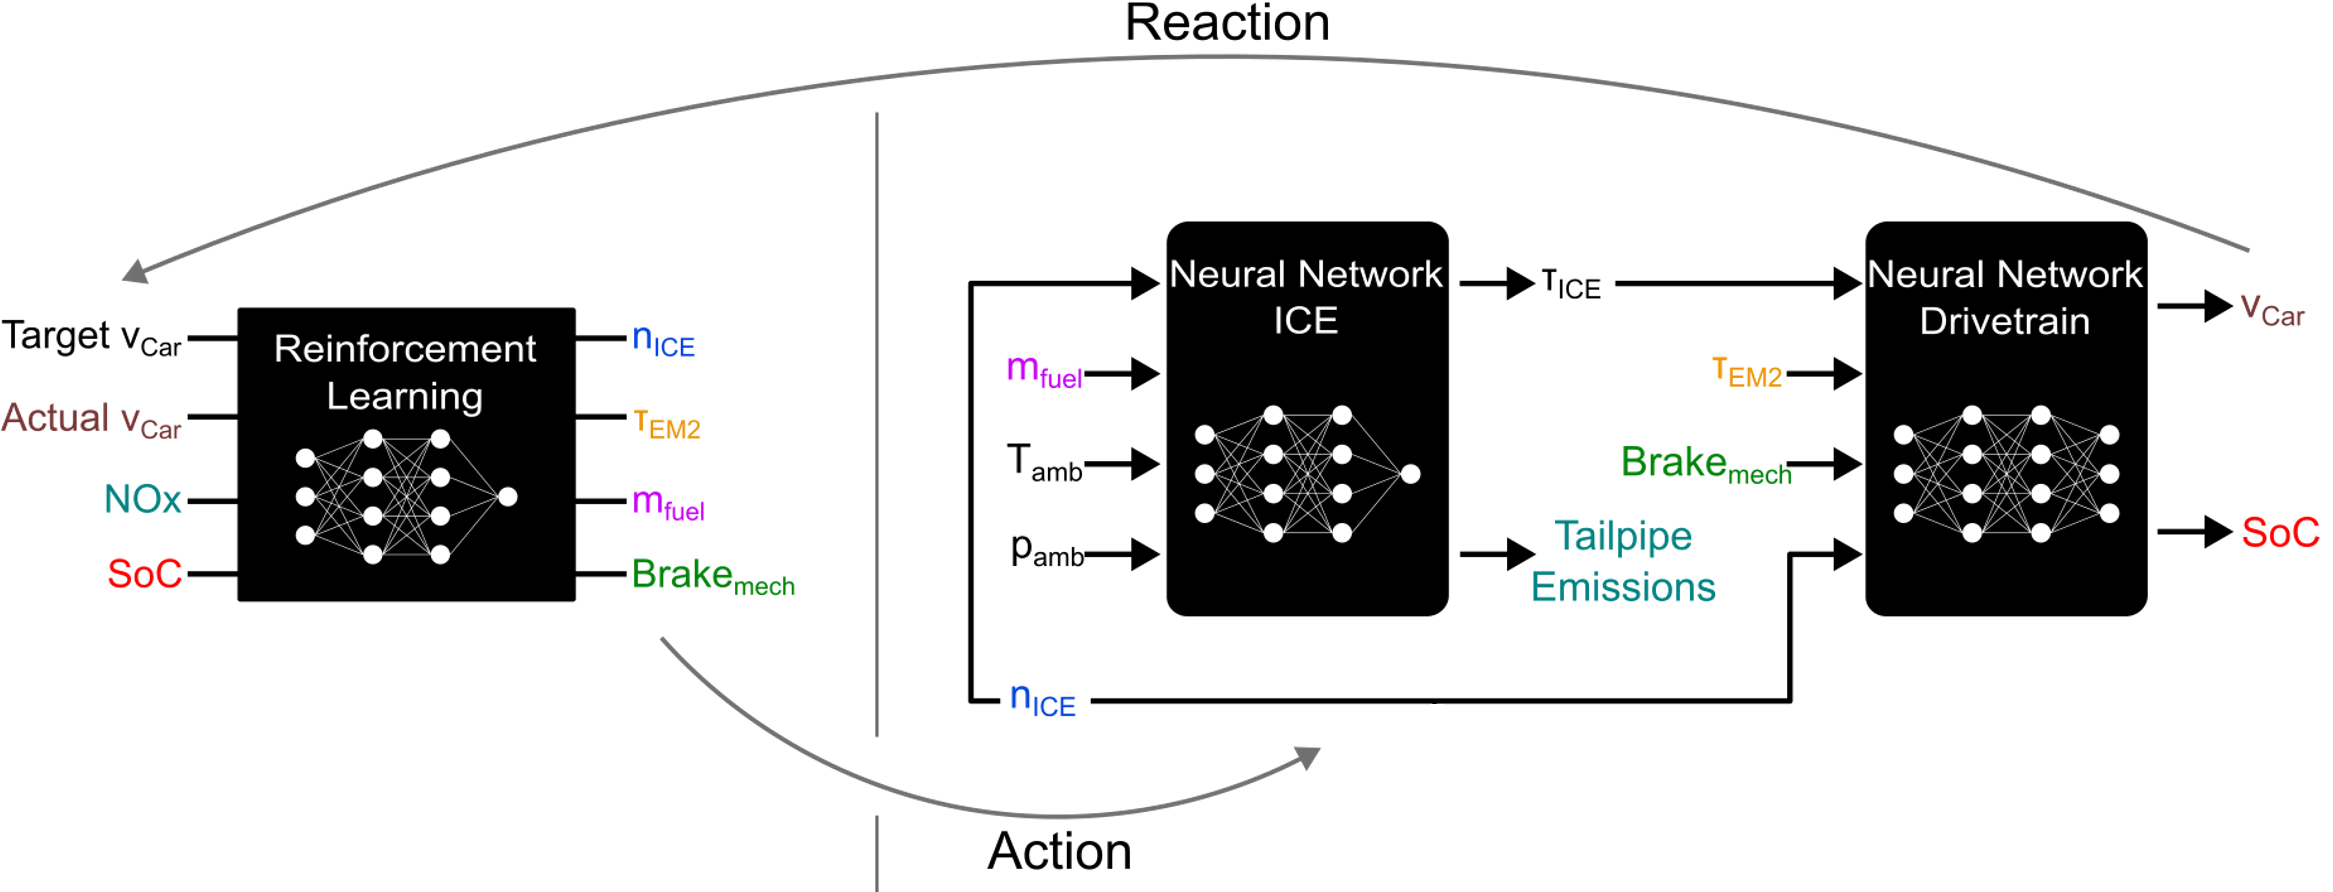
\includegraphics[width=0.9\textwidth]{imgs/control_flow.png}
  \caption[Closed-loop surrogate-environment interaction]{Closed-loop interaction between the \ac{RL} agent and the surrogate environment.}
  \label{fig:control_loop}
\end{figure}

The overall control loop consists of an \ac{RL} agent interacting with a surrogate \ac{HEV} environment, as shown in \autoref{fig:control_loop}. The environment is composed of two cascaded \ac{LSTM} models: an \ac{ICE} surrogate, which predicts engine torque and emissions, and a drivetrain surrogate, which uses the predicted torque together with the remaining actuator commands to predict vehicle speed and \ac{SOC}.

% The initially considered observations, actions and surrogate-model interfaces are summarised in \autoref{tab:control_loop_io}.

% \begin{table}[H]
%   \centering
%   \small
%   \begin{tabular}{|p{0.24\textwidth}|p{0.34\textwidth}|p{0.34\textwidth}|}
%     \hline
%     \textbf{Loop Element} & \textbf{Inputs / Observations} & \textbf{Outputs / Actions} \\
%     \hline
%     \ac{RL} Agent & Target velocity ($v_{\mathrm{target}}$), actual vehicle velocity ($v_{Car}$), tailpipe \ac{NOx} mass-flow rate ($\dot m_{\mathrm{NO}_{x},\mathrm{tp}}$), \ac{SOC} ($SoC$) & \ac{ICE} speed ($n_{ICE}$), \ac{EM2} torque ($\tau_{EM2}$), fuel mass ($m_{fuel}$), mechanical brake percentage (\texttt{Brakemech}) \\
%     \hline
%     \ac{ICE} Surrogate & Fuel mass ($m_{fuel}$), \ac{ICE} speed ($n_{ICE}$), ambient temperature ($T_{amb}$), ambient pressure ($p_{amb}$) & Tailpipe \ac{NOx} mass-flow rate ($\dot m_{\mathrm{NO}_{x},\mathrm{tp}}$), \ac{ICE} torque ($\tau_{ICE}$) \\
%     \hline
%     Drivetrain Surrogate & \ac{ICE} torque ($\tau_{ICE}$), \ac{EM2} torque ($\tau_{EM2}$), mechanical brake percentage (\texttt{Brakemech}), \ac{ICE} speed ($n_{ICE}$) & Actual vehicle velocity ($v_{Car}$), \ac{SOC} ($SoC$) \\
%     \hline
%   \end{tabular}
%   \caption[Surrogate-environment inputs and outputs]{Initially considered inputs and outputs of the closed-loop surrogate environment.}
%   \label{tab:control_loop_io}
% \end{table}

Earlier work within the \ac{LDCI2027} project used a recurrent \ac{TD3} algorithm as the \ac{RL} agent and correctly framed the control problem as a \ac{POMDP}; however, it was not able to stabilise the vehicle speed at a single constant target value (see \autoref{chap:related_work}). This thesis therefore adopts a simplified formulation to obtain stable control behaviour, while explicitly acknowledging that the underlying \ac{POMDP} is not handled optimally: it uses non-recurrent agents, approximates the partially observable problem as an \ac{MDP}, and extends the control objective from maintaining one fixed speed to tracking a complete speed trajectory.

% ---------------------------------------------------------------------
\section{Reinforcement Learning Problem Formulation}
\label{sec:method_rl_formulation}
Again, the task is formulated as a \ac{RL} problem in which an agent interacts with an environment represented by two \ac{LSTM} surrogate models representing the \ac{ICE} and the drivetrain. As discussed in \autoref{subsec:simulation_hevs}, these models replace more expensive physical simulations while preserving the temporal structure required for control development.

\subsection{Markov Decision Process Framing}
\label{subsec:method_mdp}
The problem formulation is inherently partially observable. The plant models contain internal states that capture thermal engine and aftertreatment dynamics, but these states would not be directly measurable in a deployed vehicle with the assumed sensor setup. The control problem is therefore more accurately described as a partially observable sequential decision problem than as a fully observable one.

At the current stage of development, however, these thermal effects are represented only in simplified form to reduce complexity. A more rigorous treatment of the hidden internal state would require recurrent \ac{RL} algorithms, which can use \ac{LSTM}s or other recurrent neural networks to infer latent plant dynamics. This thesis does not take that step. Although the \ac{LSTM} surrogates expose several aftertreatment-related variables, only one thermal value is included in the agent's observation vector: the temperature of \ac{SCR}1. This variable serves as a partial proxy for the otherwise hidden thermal state and allows the problem to be approximated as an \ac{MDP} for the present implementation, even though the real system is more accurately characterised as a \ac{POMDP}.

% [EXISTS, finish] resolve the note below: spell out WHICH parts make it a
% POMDP, what is respected vs. ignored, and HOW exactly it is framed as an MDP.

\subsection{Observation Design}
\label{subsec:method_observation}
% [NEW, conceptual] WHAT the agent senses and the governing rule: only
% quantities plausibly measurable on a real vehicle. Group conceptually:
% tracking error, powertrain state, ONE thermal proxy (SCR1 wall temp),
% last actions. WHY each group is included.
% -> Exact 12-dim vector + physical bounds + min-max normalisation: Impl 4.3.

The observation supplied to the agent is intentionally extensive, but it remains restricted to quantities that could plausibly be measured on a real vehicle with a realistic sensor setup. Consequently, the internal recurrent states of the plant models and most aftertreatment temperatures are excluded, even though the surrogate networks would expose them, because they would not be available at deployment time. Within this constraint, the observation comprises four conceptual groups:

\begin{itemize}
  \item \textbf{Tracking information.} The current vehicle speed and its error relative to the reference trajectory, which define the primary tracking objective.
  \item \textbf{Energy state.} The battery \ac{SOC} and its deviation from the initial value, which provide the information required for charge-sustaining operation.
  \item \textbf{Powertrain and emission state.} Instantaneous quantities such as \ac{ICE} speed, \ac{ICE} torque, injected fuel mass and tailpipe \ac{NOx}, which characterise the current engine operating point and its immediate emission consequence.
  \item \textbf{Actuation history.} The most recent actuator commands and a normalised timer counting the steps since the last engine on/off transition, which provide limited temporal context for the otherwise memoryless policy.
\end{itemize}

A single thermal variable, the wall temperature of the \ac{SCR} before the turbine, is included as a deliberate exception. It serves as a partial proxy for the otherwise hidden aftertreatment thermal state and is the only concession used to approximate the underlying \ac{POMDP} as the tractable \ac{MDP} formulation adopted in this thesis (\autoref{subsec:method_mdp}). Other potentially useful variables that would not be measurable on a real vehicle are excluded by design. The exact composition of the observation vector, the physical bounds of each component and the per-component normalisation applied before the policy network are reported in \autoref{sec:impl_environment}.

\subsection{Action Design}
\label{subsec:method_action}
% [NEW, conceptual] WHAT the agent controls: engine on/off + speed, EM2
% torque, fuel mass, brake. Conceptual choice: a single CONTINUOUS engine
% command encoding both the on/off decision and the rpm setpoint.
% [SHIFT] The 900-rpm invalid region is handled here by command ENCODING +
% a minimum-dwell rule, in contrast to the prior project's differentiable
% sigmoid "soft-gate" layers (see Related Work).
% -> Exact rescaling / mapping (<=0 -> off; >0 -> 900..4000 rpm): Impl 4.3.
The action design is based on the requirements specified by the \ac{LDCI2027} project \cite{universitat_politecnica_de_catalunya_development_2025}. At the conceptual level, the controller must output four control quantities (see~\autoref{fig:control_loop}):
\begin{itemize}
  \item \ac{ICE} speed ($n_{ICE}$),
  \item \ac{EM2} torque ($\tau_{EM2}$),
  \item fuel mass ($m_{fuel}$), and
  \item mechanical brake percentage (\texttt{Brakemech}).
\end{itemize}

These quantities describe the required control interfaces, but they do not fully capture the input restrictions imposed by the plant \ac{LSTM}s. In particular, the engine has two distinct operating regimes: an engine-off state and an engine-on state with a valid \ac{ICE} speed and fuel mass interval. An explicit engine-off case therefore has to be represented in the action design. While the earlier \ac{LDCI2027} work incorporated sigmoid soft-gate layers for this purpose \cite{universitat_politecnica_de_catalunya_development_2025} (see \autoref{chap:related_work}), this thesis uses a single continuous engine command as the corresponding agent action. Internally, this command is then mapped either to the engine-off case or to a valid engine-on \ac{ICE} speed and fuel mass range.

\subsection{Reward Design}
\label{subsec:method_reward}
% [NEW, conceptual] Gaussian speed-tracking core (dense, bounded, peak at
% zero error) + penalty terms for NOx / SOC / fuel / brake / engine-flicker.
% WHY a shaped reward at all; introduce the principle of optimising the TRUE
% objective (speed RMSE) rather than the reward proxy.
% -> Exact formula, normalisation factors and weights: Impl 4.3 / Results.

The reward is the channel through which the control objectives are communicated to the agent. It combines a primary speed-tracking term with penalty terms for the secondary objectives, namely emissions and \ac{SOC} deviation, as well as a small number of shaping terms for mechanically undesirable behaviour such as unnecessary braking and rapid engine on/off switching. The speed-tracking reward is maximal at zero tracking error and decays smoothly as the error increases.

Because the objectives are measured on very different physical scales (e.g. km/h vs grams), each term is normalised to a comparable range before weighting. This keeps the relative weights interpretable and prevents any single objective from overwhelming the others. Such behaviour was observed in an earlier iteration of the project, where an unnormalised emission penalty dominated the \ac{SOC} reward and prevented the agent from converging (\autoref{chap:related_work}). The shaping terms are kept small because they are intended to regularise implausible actuation and guide learning, rather than to express primary objectives in their own right.

Since the \ac{RL} reward is a proxy for the true objectives rather than the objective itself, agents are selected and compared using directly measured deployment metrics (\autoref{sec:method_evaluation}), not accumulated reward. Enabling or disabling individual terms through their weights also realises the staged learning approach: Phase~1 keeps only the speed-tracking term active, whereas Phase~2 additionally activates the emission and \ac{SOC} terms (\autoref{subsec:method_phase1}, \autoref{subsec:method_phase2}). The exact reward formulation, normalisation factors and per-phase weights are given in \autoref{sec:impl_environment}.

\subsection{Selection of Reinforcement-Learning Algorithms}
\label{subsec:method_algo_selection}
% [NEW] WHY model-free actor-critic for continuous control; PPO = simple
% on-policy baseline / sanity check to get training running; SAC + TD3 =
% off-policy, sample-efficient. Tie to Related Work (SAC ~ Tresca, TD3 ~ Zhou)
% and to prior-project experience.
% -> Algorithm MECHANICS belong in Theory (Ch.2); SB3 configs in Impl 4.4.

The final selection of \ac{RL} algorithms was guided by two considerations:

\begin{itemize}
  \item First, a simple and widely used baseline algorithm was needed to verify that the training pipeline and environment interaction worked as intended. \ac{PPO} was selected for this role because it is comparatively easy to understand, well documented and commonly implemented.
  \item Second, more capable off-policy algorithms were required for the main continuous-control experiments. \ac{SAC} and \ac{TD3} were selected because they are sample-efficient actor--critic methods and have been used successfully in related \ac{HEV} control studies: \cite{tresca_cutting-edge_2025} used \ac{SAC}, while \cite{zhou_novel_2021} used \ac{TD3}. They also align with the prior \ac{LDCI2027} work, in which \ac{SAC} was used in \cite{cuberos_munoz_developing_2025} and (recurrent) \ac{TD3} was used in \cite{universitat_politecnica_de_catalunya_development_2025}. These algorithms therefore provide the more advanced candidates for the nonlinear control task considered in this thesis.
\end{itemize}

% ---------------------------------------------------------------------
\section{Multi-Stage Course Learning Approach}
\label{sec:method_staged}
The experimental strategy follows a phase-wise procedure that is conceptually close to curriculum learning \cite{bengio_curriculum_2009}. It separates basic controllability from later multi-objective optimisation and thereby makes the validation process more interpretable.

\begin{figure}[htbp]
  \centering
  \includestandalone[width=\textwidth]{tikz/overall_methodology}
  \caption[Overall experimental pipeline of the study]{Overall experimental pipeline of the study.}
  \label{fig:overall_methodology}
\end{figure}

\subsection{Terminology and Motivation}
\label{subsec:method_staged_terminology}
Training a \ac{DRL} agent on conflicting multi-objective goals simultaneously, as is the case in controlling an \ac{HEV}, is a difficult problem and can lead to local optima and unstable training. Learning such complex and nonlinear control policies therefore requires additional guidance to stabilise training. Optimising several variables at once increases the complexity of the problem, according to the curse of dimensionality (see \autoref{sec:problem_description}), and contributed to the difficulty of balancing reward weights in the prior \ac{LDCI2027} work \cite{cuberos_munoz_developing_2025}. This thesis addresses this issue by implementing a \textit{multi-stage course-learning approach}. Although this term is adopted from Wang and Wang \cite{wang_energy_2025}, it describes the broader concept of curriculum learning in machine learning \cite{bengio_curriculum_2009}, where the difficulty of the learning task is increased as the model's competence improves. Sutton and Barto \cite{sutton_reinforcement_2020} however refer to this technique as \textit{shaping}. Derived from animal psychology, shaping involves ``changing the reward signal as learning proceeds'' \cite{sutton_reinforcement_2020}.

In this thesis, the term \textit{shaping} follows Ibrahim et al. \cite{ibrahim_comprehensive_2024} and should not be confused with Sutton and Barto's use of the term. Here, shaping is understood in the context of reward shaping: reward engineering defines the reward function itself, whereas reward shaping further refines or augments the reward signal to guide learning more effectively \cite{ibrahim_comprehensive_2024}. The concrete reward design used in this work is described in \autoref{subsec:method_reward} and implemented in \autoref{sec:impl_environment}.

In the first phase, the reward function is designed to prioritise the fundamental prerequisite of speed tracking. Once baseline control competence has been established, the trained models are reused and the curriculum advances to a second stage, in which additional reward terms for \ac{SOC} deviation and \ac{NOx} emissions are activated to optimise the energy-management strategy. This simplifies the learning process by addressing the objectives sequentially rather than all at once, thereby reducing the complexity of the optimisation problem.

\subsection{Phase 1 — Exclusive Speed Tracking}
\label{subsec:method_phase1}
The agents are trained with a single active objective - speed tracking. In this stage, \ac{PPO}, \ac{TD3} and \ac{SAC} are each expected to learn how to follow the desired speed profile as accurately as possible, while effects on battery \ac{SOC} and emissions are deliberately ignored in the reward. The results are used to record the corresponding \ac{SOC} variation and \ac{NOx} emission levels, establishing empirical reference bounds for the later optimisation stage.

\paragraph{The two questions Phase~1 answers.}
The role of Phase~1 in the overall thesis goal of learning a speed-tracking and emission-reducing controller for an HEV is twofold:

\begin{enumerate}
  \item \textbf{Feasibility.} Demonstrate that each candidate \ac{RL} algorithm can learn the speed-tracking task at all in the \ac{LSTM}-surrogate environment, thereby ruling out environment-side training issues before any reward extension is attempted.
  \item \textbf{Unconstrained baselines.} Quantify the cumulative \ac{NOx} emissions and the \ac{SOC} drift that emerge as side effects of speed-only optimisation. These two quantities are the targets that Phase~2 must improve upon and define the reference against which any multi-objective formulation will be benchmarked.
\end{enumerate}

\subsection{Phase 2 — Multi-Objective Optimisation}
\label{subsec:method_phase2}
Phase~2 fine-tunes the best Phase~1 checkpoint (the one with the lowest RMSE in speed-tracking), selected from the ten seed runs, under an augmented multi-objective reward. In addition to speed tracking, the reward activates \ac{NOx} and \ac{SOC} terms. The objective is therefore not merely to follow the speed trajectory, but to do so with lower tailpipe \ac{NOx} emissions while avoiding the trivial strategy of depleting the battery. Phase~2 addresses this directly by steering the policy towards charge-sustaining, low-emission operation without discarding the tracking behaviour learned in Phase~1.

\paragraph{Fine-tuning from the Phase~1 checkpoint.} Rather than training each agent from scratch under the full multi-objective reward, Phase~2 initialises every agent from its Phase~1 best-seed checkpoint and fine-tunes it under the augmented reward. Conceptually, this transfers the already-learned speed-tracking behaviour into the second stage, so that training only has to reshape the policy towards the additional objectives instead of re-learning controllability from zero. This warm-start is the core of the curriculum-inspired staged approach: basic controllability is acquired first and the harder multi-objective trade-off is introduced only once that foundation is in place.

\paragraph{Reward augmentation.}
The augmented reward retains the Phase~1 speed-tracking term and adds two penalties. The first penalises tailpipe \ac{NOx}, reflecting the central objective of the thesis. The second penalises deviations of the battery \ac{SOC} from its initial value, enforcing charge-sustaining behaviour. The exact reward formulation and weights are reported in \autoref{sec:impl_environment}.

The main difficulty in Phase~2 is balancing the conflicting objectives of speed tracking, emission reduction and charge sustainment. Their relative importance is controlled by the reward weights. Two strategies for selecting these weights are considered. The first is a manual grid search over the emission and \ac{SOC} weights, with one agent fine-tuned for each combination. This approach is simple and interpretable, but it evaluates only a small number of fixed combinations at substantial computational cost.

\paragraph{Tuning reward weights.} The grid search is therefore replaced by an automated Optuna search using the sampling and pruning strategy already employed in Phase~1. Each trial fine-tunes an agent with a sampled weight pair and evaluates it using a \emph{composite score} that reflects the intended behaviour: minimise cumulative tailpipe \ac{NOx}, while applying increasing penalties when speed-tracking error or battery drift exceed acceptable tolerances. This converts the multi-objective trade-off into a constrained scalar objective and focuses the search on weight regions that reduce emissions without sacrificing tracking or charge sustainment. The exact weight ranges, penalty tolerances and search budget are given in \autoref{subsec:impl_phase2_pipeline}.

Overall, Phase~2 measures how far optimised multi-objective policy improves over the baselines established in Phase~1.

% ---------------------------------------------------------------------
\section{Evaluation Methodology}
\label{sec:method_evaluation}
The evaluation of both, Phase~1 and Phase~2 follows deliberate protocols:

\paragraph{True objective versus reward proxy for Phase~1.}
% Models are selected / compared on measured speed RMSE, NOT on episodic
% shaped reward (the reward only encodes the objective approximately).
As discussed above, the reward signal is only a proxy for the real task objective. Although cumulative reward is commonly used to evaluate \ac{RL} agents \cite{sutton_reinforcement_2020}, it can be misleading when the reward function is imperfectly designed. This is particularly relevant in Phase~1, where the target objective is explicitly defined as speed tracking only. The best Phase~1 agent is therefore not selected by the highest cumulative reward, but by the lowest \ac{RMSE} between the target speed trajectory and the realised vehicle speed. The \ac{RMSE} is defined as

\begin{equation}
  \mathrm{RMSE}_v = \sqrt{\frac{1}{N}\sum_{t=1}^{N}\left(v_{\mathrm{target},t} - v_{Car,t}\right)^2},
\end{equation}
where $N$ is the number of evaluated time steps, $v_{\mathrm{target},t}$ is the target velocity at time step $t$, and $v_{Car,t}$ is the corresponding realised vehicle velocity.

\paragraph{Performance metrics.}
Phase~1 therefore uses speed-tracking \ac{RMSE} [km/h] as its primary performance metric. It also records cumulative \ac{NOx} emissions [g/evaluation cycle], battery \ac{SOC} drift [decimal fraction], and cumulative fuel consumption [g/evaluation cycle] as diagnostic quantities. The \ac{SOC} drift is reported as the absolute difference between the initial and final \ac{SOC} values. Speed-tracking \ac{MAE} [km/h] is included as an additional tracking metric: while \ac{MAE} weights all absolute speed errors linearly, \ac{RMSE} penalises larger deviations more strongly because the errors are squared before averaging. Consequently, \ac{RMSE} is used as the main Phase~1 selection criterion, whereas Phase~2 combines speed-tracking \ac{RMSE}, cumulative \ac{NOx}, and \ac{SOC} drift into a composite scalar score. The exact formulation is given in \autoref{subsec:impl_phase2_pipeline}.

\paragraph{Statistical reliability.}
To account for the stochastic nature of \ac{DRL}, each selected configuration is trained and evaluated with multiple random seeds. The resulting metrics are reported as mean $\pm$ standard deviation across seeds, which makes it possible to distinguish systematic algorithm behaviour from random-seed variance. In addition to these aggregate statistics, the best-performing seed is retained as the checkpoint for the subsequent phase, since Phase~2 requires a single policy to be fine-tuned.

\paragraph{Evaluation cycle.}
Each trained policy is evaluated on the standardised six-phase speed trajectory shown in \autoref{fig:six_phase_trajectory}. Inference is performed deterministically to ensure reproducibility and comparability. The speed steps are defined heuristically to assess acceleration and deceleration at different intensities. The implementation can also be applied to other trajectories, including synthetic cycles, standardised real-world driving cycles, and constant-speed scenarios.

\begin{figure}[htbp]
  \centering
  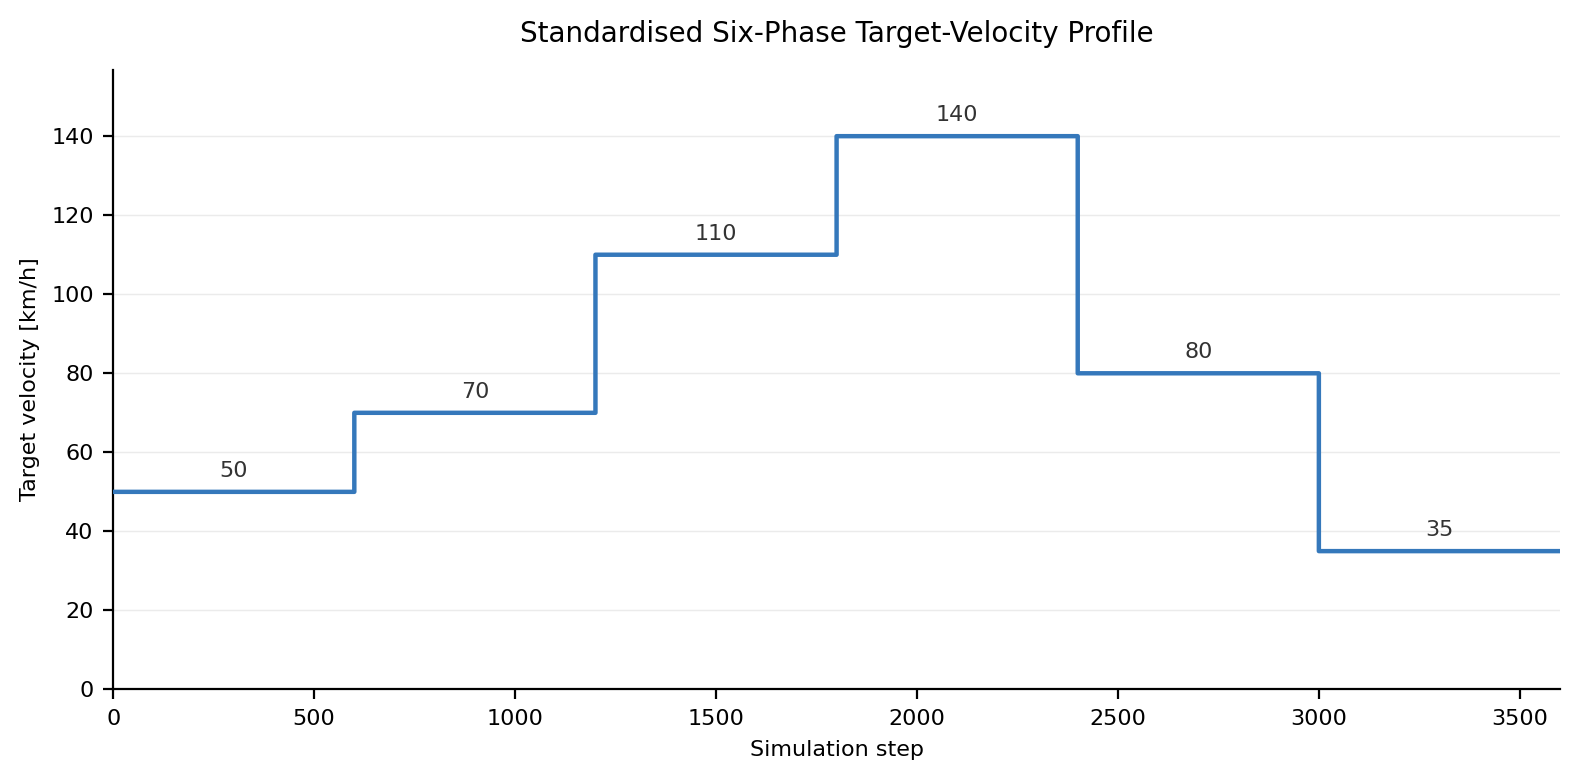
\includegraphics[width=0.65\textwidth]{imgs/eval_target_profile.png}
  \caption[Six-phase target-velocity trajectory]{Standardised six-phase target-velocity trajectory used as the default evaluation benchmark.}
  \label{fig:six_phase_trajectory}
\end{figure}

\paragraph{Final WLTC comparison.}
While phase 1 and phase 2 both evaluate their hyperparameter or reward tuning experiments on the same evaluation cycle (\autoref{fig:six_phase_trajectory}), a final experiment is conducted which switches the evaluation cycle from the synthetic one to a real-world standardised \ac{WLTC} \cite{united_nations_economic_commission_for_europe_global_2014}. The \ac{WLTC} is a globally standardised driving profile used to measure automotive fuel consumption, tailpipe emissions, and electric vehicle range. Derived from real-world driving data, it consists of distinct low, medium, high, and extra-high speed phases that mimic diverse urban, suburban, rural, and motorway driving conditions.

This final comparison is used to bridge the gap simulation to reality gap a bit more by assessing the learned controller in a more realistic scenario instead exclusively on synthetic cycles. It assesses the capability of the final models to generalise to sitation that havent been part of their training and compares the effectivity of them, in terms of speed tracking, \ac{NOx} reduction and \ac{SOC} sustainment compared to a rule-based solution developed by Frey et al. \cite{frey_data-based_2025}.
